\section{Imágenes}
En \LaTeX, las imágenes se pueden incluir utilizando el paquete \texttt{graphicx}. 
Para añadir una imagen en texstudio, es posible arrastrarla directamente en el editor, lo que obtendrá como resultado lo mostrado en la \autoref{fig:insertarimagen}.

\begin{figure}[h]
	\centering
	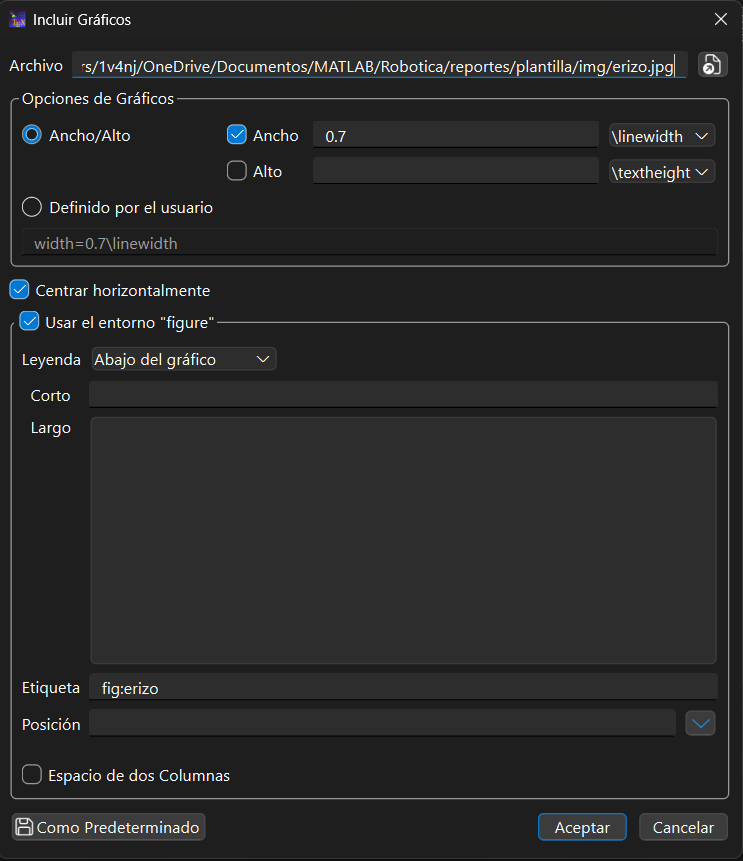
\includegraphics[width=0.7\linewidth]{img/insertarImagen}
	\caption{Opciones al insertar una imagen}
	\label{fig:insertarimagen}
\end{figure}

Algunas opciones clave incluyen:

\begin{itemize}
	\item \textbf{Tamaño de la imagen}: Se puede definir un ancho o alto relativo a la caja de texto o se puede usar un tamaño en pixeles (px), centímetros (cm) o el ancho de la letra M (em).
	\item \textbf{Centrado}: Se puede marcar la opción para que la imagen aparezca centrada automáticamente.
	\item \textbf{Uso del entorno `figure'}: Permite que la imagen tenga una numeración automática y pueda referenciarse en el texto con \texttt{\textbackslash ref\{\}} o \texttt{\textbackslash autoref\{\}}.
	\item \textbf{Posicionamiento (`h`, `t`, `b`, `p`)}: Al presionar la flecha de la derecha, podemos añadir las opciones que determinan la posición de la imagen en el documento, como después del texto o arriba de la página, etc. Si igual vamos a referenciar las figuras, es innecesario que estén exactamente donde fueron mencionadas ya que eso deja muchos espacios en blanco.
	\item \textbf{Leyenda Largo}: permite poner una descripción de la imagen en el lugar que elegimos (debería de estar debajo).
	\item \textbf{Etiqueta}: nos servirá para referenciarla. 
\end{itemize}

Para usar dos imágenes como en \autoref{fig:mascotas}, se utilizó \texttt{subfloat}.
% Dos imágenes de mascotas
\begin{figure}[h]
	\centering
	\subfloat[Perro]{%
		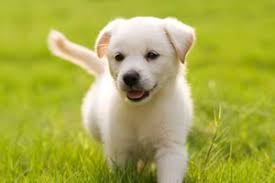
\includegraphics[width=0.4\textwidth]{perro.jpg}%
		\label{fig:perro}
	}
	\hfill
	\subfloat[Gato]{%
		
\includegraphics[width=0.4\textwidth]{gato.jpg}%
		\label{fig:gato}
	}
	\caption{Imagen de dos mascotas}
	\label{fig:mascotas}
\end{figure}